\chapter{Solving DSGE models - basics} \label{ch:solbase}

This chapter covers everything that leads to, and stems from, the solution of DSGE models; a vast terrain. That is to say that the term ``solution'' in the title of the chapter is used rather broadly. You may be interested in simply finding the solution functions to a set of first order conditions stemming from your model, but you may also want to go a bit further. Typically, you may be interested in how this system behaves in response to shocks, whether temporary or permanent. Likewise, you may want to explore how the system comes back to its steady state or moves to a new one. This chapter covers all these topics. But instead of skipping to the topic closest to your needs, we recommend that you read this chapter chronologically, to learn basic Dynare commands and the process of writing a proper .mod file - this will serve as a base to carry out any of the above computations. 

\section{A fundamental distinction} \label{sec:distcn}
Before speaking of Dynare, it is important to recognize a distinction in model types. This distinction will appear throughout the chapter; in fact, it is so fundamental, that we considered writing separate chapters altogether. But the amount of common material - Dynare commands and syntax - is notable and writing two chapters would have been overly repetitive. Enough suspense; here is the important question: \textbf{is your model stochastic or deterministic?}\\

The distinction hinges on \textbf{whether future shocks are known}. In deterministic models, the occurrence of all future shocks is known exactly at the time of computing the model's solution. In stochastic models, instead, only the distribution of future shocks is known. Let's consider a shock to a model's innovation only in period 1. In a deterministic context, agents will take their decisions knowing that future values of the innovations will be zero in all periods to come. In a stochastic context, agents will take their decisions knowing that the future value of innovations are random but will have zero mean. This isn't the same thing because of Jensen's inequality. Of course, if you consider only a first order linear approximation of the stochastic model, or a linear model, the two cases become practically the same, due to certainty equivalence. A second order approximation will instead lead to very different results, as the variance of shocks will matter. \\

The solution method for each of these model types differs significantly. In deterministic models, a highly accurate solution can be found by numerical methods. The solution is nothing more than a series of numbers that match a given set of equations. Intuitively, if an agent has perfect foresight, she can specify today - at the time of making her decision - what each of her precise actions will be in the future. In a stochastic environment, instead, the best the agent can do is specify a decision, policy or feedback rule for the future: what will her optimal actions be contingent on each possible realization of shocks. In this case, we therefore search for a function satisfying the model's first order conditions. To complicate things, this function may be non-linear and thus needs to be approximated. In control theory, solutions to deterministic models are usually called ``closed loop'' solutions, and those to stochastic models are referred to as ``open loop''.\\

Because this distinction will resurface again and again throughout the chapter, but also because it has been a source of significant confusion in the past, the following gives some additional details. 

\subsection{\textsf{NOTE!} Deterministic vs stochastic models} \label{sec:detstoch}

\textbf{Deterministic} models have the following characteristics:
\begin{enumerate}
\item As the DSGE (read, ``stochastic'', i.e. not deterministic!) literature has gained attention in economics, deterministic models have become somewhat rare. Examples include OLG models without aggregate uncertainty.
\item These models are usually introduced to study the impact of a change in regime, as in the introduction of a new tax, for instance. 
\item Models assume full information, perfect foresight and no uncertainty around shocks.
\item Shocks can hit the economy today or at any time in the future, in which case they would be expected with perfect foresight. They can also last one or several periods.
\item Most often, though, models introduce a positive shock today and zero shocks thereafter (with certainty).
\item The solution does not require linearization, in fact, it doesn't even really need a steady state. Instead, it involves numerical simulation to find the exact paths of endogenous variables that meet the model's first order conditions and shock structure. 
\item This solution method can therefore be useful when the economy is far away from steady state (when linearization offers a poor approximation).
\end{enumerate}
\textbf{Stochastic} models, instead, have the following characteristics:
\begin{enumerate}
\item These types of models tend to be more popular in the literature. Examples include most RBC models, or new keynesian monetary models.
\item In these models, shocks hit today (with a surprise), but thereafter their expected value is zero. Expected future shocks, or permanent changes in the exogenous variables cannot be handled due to the use of Taylor approximations around a steady state.
\item Note that when these models are linearized to the first order, agents behave as if future shocks where equal to zero (since their expectation is null), which is the \textbf{certainty equivalence property}. This is an often overlooked point in the literature which misleads readers in supposing their models may be deterministic.
\end{enumerate}


\section{Introducing an example}
The goal of this first section is to introduce a simple example. Future sections will aim to code this example into Dynare and analyze its salient features under the influence of shocks - both in a stochastic and a deterministic environment. Note that as a general rule, the examples in the basic chapters, \ref{ch:solbase} and \ref{ch:estbase}, are kept as bare as possible, with just enough features to help illustrate Dynare commands and functionalities. More complex examples are instead presented in the advanced chapters.\\

The model introduced here is a basic RBC model with monopolistic competition, used widely in the literature. Its particular notation adopted below is drawn mostly from notes available on Jesus Fernandez-Villaverde's very instructive \href{http://www.econ.upenn.edu/~jesusfv/}{website}; this is a good place to look for additional information on any of the following model set-up and discussion. Note throughout this model description that the use of \textbf{expectation} signs is really only relevant in a stochastic setting, as per the earlier discussion. We will none-the-less illustrate both the stochastic and the deterministic settings on the basis of this example. Thus, when thinking of the latter, you'll have to use a bit of imagination (on top of that needed to think you have perfect foresight!) to ignore the expectation signs.\\

Households maximize utility over consumption, $c_t$ and leisure, $1-l_t$, where $l_t$ is labor input, according to the following utility function
\[
\mathbb{E}_t \sum_{t=0}^{\infty} \beta \left[ \log c_t + \psi \log(1-l_t) \right]
\]
and subject to the following budget constraint
\[
c_t + k_{t+1}=w_t l_t + r_t k_t + (1-\delta)k_t, \qquad \forall t>0
\]
where $k_t$ is capital stock, $w_t$ real wages, $r_t$ real interest rates or cost of capital and $\delta$ the depreciation rate. \\

The above equation can be seen as an accounting identity, with total expenditures on the left hand side and revenues - including the liquidation value of the capital stock - on the right hand side. Alternatively, with a little more imagination, the equation can also be interpreted as a capital accumulation equation after bringing $c_t$ to the right hand side and noticing that $w_t l_t + r_t k_t$, total payments to factors, equals $y_t$, or aggregate output, by the zero profit condition. As a consequence, if we define investment as $i_t=y_t - c_t$, we obtain the intuitive result that $i_t=k_{t+1} - (1-\delta) k_{t}$, or that investment replenishes the capital stock thereby countering the effects of depreciation. In any given period, the consumer therefore faces a tradeoff between consuming and investing in order to increase the capital stock and consuming more in following periods (as we will see later, production depends on capital).\\

Maximization of the household problem with respect to consumption, leisure and capital stock, yields the Euler equation in consumption, capturing the intertemporal tradeoff mentioned above, and the labor supply equation linking labor positively to wages and negatively to consumption (the wealthier, the more leisure due to the decreasing marginal utility of consumption). These equation are
\[
\frac{1}{c_t}=\beta \mathbb{E}_t \left[ \frac{1}{c_{t+1}} \left( 1 + r_{t+1} - \delta \right) \right]
\]
and
\[
\psi \frac{c_t}{1-l_t}= w_t
\]

The firm side of the problem is slightly more involved, due to monopolistic competition, but is presented below in the simplest possible terms, with a little hand-waiving involved, as the derivations are relatively standard. \\

There are two ways to introduce monopolistic competition. We can either assume that firms sell differentiated varieties of a good to consumers who aggregate these according to a CES index. Or we can postulate that there is a continuum of intermediate producers with market power who each sell a different variety to a competitive final goods producer whose production function is a CES aggregate of intermediate varieties.\\

If we follow the second route, the final goods producer chooses his or her optimal demand for each variety, yielding the Dixit-Stiglitz downward sloping demand curve. Intermediate producers, instead, face a two pronged decision: how much labor and capital to employ given these factors' perfectly competitive prices and how to price the variety they produce.\\

Production of intermediate goods follows a CRS production function defined as
\[
y_{it} = k_{it}^\alpha (e^{z_t} l_{it})^{1-\alpha}
\]
where the $i$ subscript stands for firm $i$ of a continuum of firms between zero and one and where $\alpha$ is the capital elasticity in the production function, with $0<\alpha<1$. Also, $z_t$ captures technology which evolves according to
\[
z_t = \rho z_{t-1} + e_t
\]
where $\rho$ is a parameter capturing the persistence of technological progress and $e_t \thicksim \mathcal{N}(0,\sigma)$. \\

The solution to the sourcing problem yields an optimal capital to labor ratio, or relationship between payments to factors:
\[
k_{it}r_t=\frac{\alpha}{1-\alpha}w_tl_{it}
\]

The solution to the pricing problem, instead, yields the well-known constant markup pricing condition of monopolistic competition:
\[
p_{it}=\frac{\epsilon}{\epsilon -1}mc_t p_t
\]
where $p_{it}$ is firm $i$'s specific price, $mc_t$ is real marginal cost and $p_t$ is the aggregate CES price or average price. An additional step simplifies this expression: symmetric firms implies that all firms charge the same price and thus $p_{it}=p_t$; we therefore have: $mc_t = (\epsilon - 1)/\epsilon$ \\

But what are marginal costs equal to? To find the answer, we combine the optimal capital to labor ratio into the production function and take advantage of its CRS property to solve for the amount of labor or capital required to produce one unit of output. The real cost of using this amount of any one factor is given by $w_tl_{it} + r_tk_{it}$ where we substitute out the payments to the other factor using again the optimal capital to labor ratio. When solving for labor, for instance, we obtain
\[
mc_t = \left( \frac{1}{1-\alpha}�\right)^{1-\alpha} \left( \frac{1}{\alpha}�\right)^\alpha \frac{1}{A_t}w_t^{1-\alpha} r_t^\alpha
\]
which does not depend on $i$; it is thus the same for all firms. \\

Interestingly, the above can be worked out, by using the optimal capital to labor ratio, to yield $w_t [(1-\alpha)y_{it}/l_{it}]^{-1}$, or $w_t \frac{\partial l_{it}}{\partial y_{it}}$, which is the definition of marginal cost: the cost in terms of labor input of producing an additional unit of output. This should not be a surprise since the optimal capital to labor ratio follows from the maximization of the production function (minus real costs) with respect to its factors. \\

Combining this result for marginal cost, as well as its counterpart in terms of capital, with the optimal pricing condition yields the final two important equations of our model
\[
w_t = (1-\alpha) \frac{y_{it}}{l_{it}} \frac{(\epsilon-1)}{\epsilon}
\]
and
\[
r_t = \alpha \frac{y_{it}}{k_{it}} \frac{(\epsilon-1)}{\epsilon}
\]

To end, we aggregate the production of each individual firm to find an aggregate production function. On the supply side, we factor out the capital to labor ratio, $k_t/l_t$, which is the same for all firms and thus does not depend on $i$. On the other side, we have the Dixit-Stiglitz demand for each variety. By equating the two and integrating both side, and noting that price dispersion is null - or that, as hinted earlier, $p_{it}=p_t$ - we obtain aggregate production
\[
y_t = A_t k_t^\alpha l_t^{1-\alpha}
\]
which can be shown is equal to the aggregate amount of varieties bought by the final good producer (according to a CES aggregation index) and, in turn, equal to the aggregate output of final good, itself equal to household consumption. Note, to close, that because the ratio of output to each factor is the same for each intermediate firm and that firm specific as well as aggregate production is CRS, we can rewrite the above two equations for $w_t$ and $r_t$ without the $i$ subscripts on the right hand side. \\

This ends the exposition of the example. Now, let's roll up our sleeves and see how we can input the model into Dynare and actually test how the model will respond to shocks. 

\section{Dynare .mod file structure}
Input into Dynare involves the .mod file, as mentioned loosely in the introduction of this Guide. The .mod file can be written in any editor, external or internal to Matlab. It will then be read by Matlab by first navigating within Matlab to the directory where the .mod file is stored and then by typing in the Matlab command line \texttt{Dynare filename.mod;} (although actually typing the extension .mod is not necessary). But before we get into executing a .mod file, let's start by writing one! \\

It is convenient to think of the .mod file as containing four distinct blocks, illustrated in figure \ref{fig:modstruct}:
\begin{itemize}
\item \textbf{preamble}: lists variables and parameters
\item \textbf{model}: spells out the model
\item \textbf{steady state or initial value}: gives indications to find the steady state of a model, or the starting point for simulations or impulse response functions based on the model's solution. 
\item \textbf{shocks}: defines the shocks to the system
\item \textbf{computation}: instructs Dynare to undertake specific operations (e.g. forecasting, estimating impulse response functions)
\end{itemize}
Our exposition below will structured according to each of these blocks. 
\begin{figure} \label{fig:modstruct}
\begin{center} 
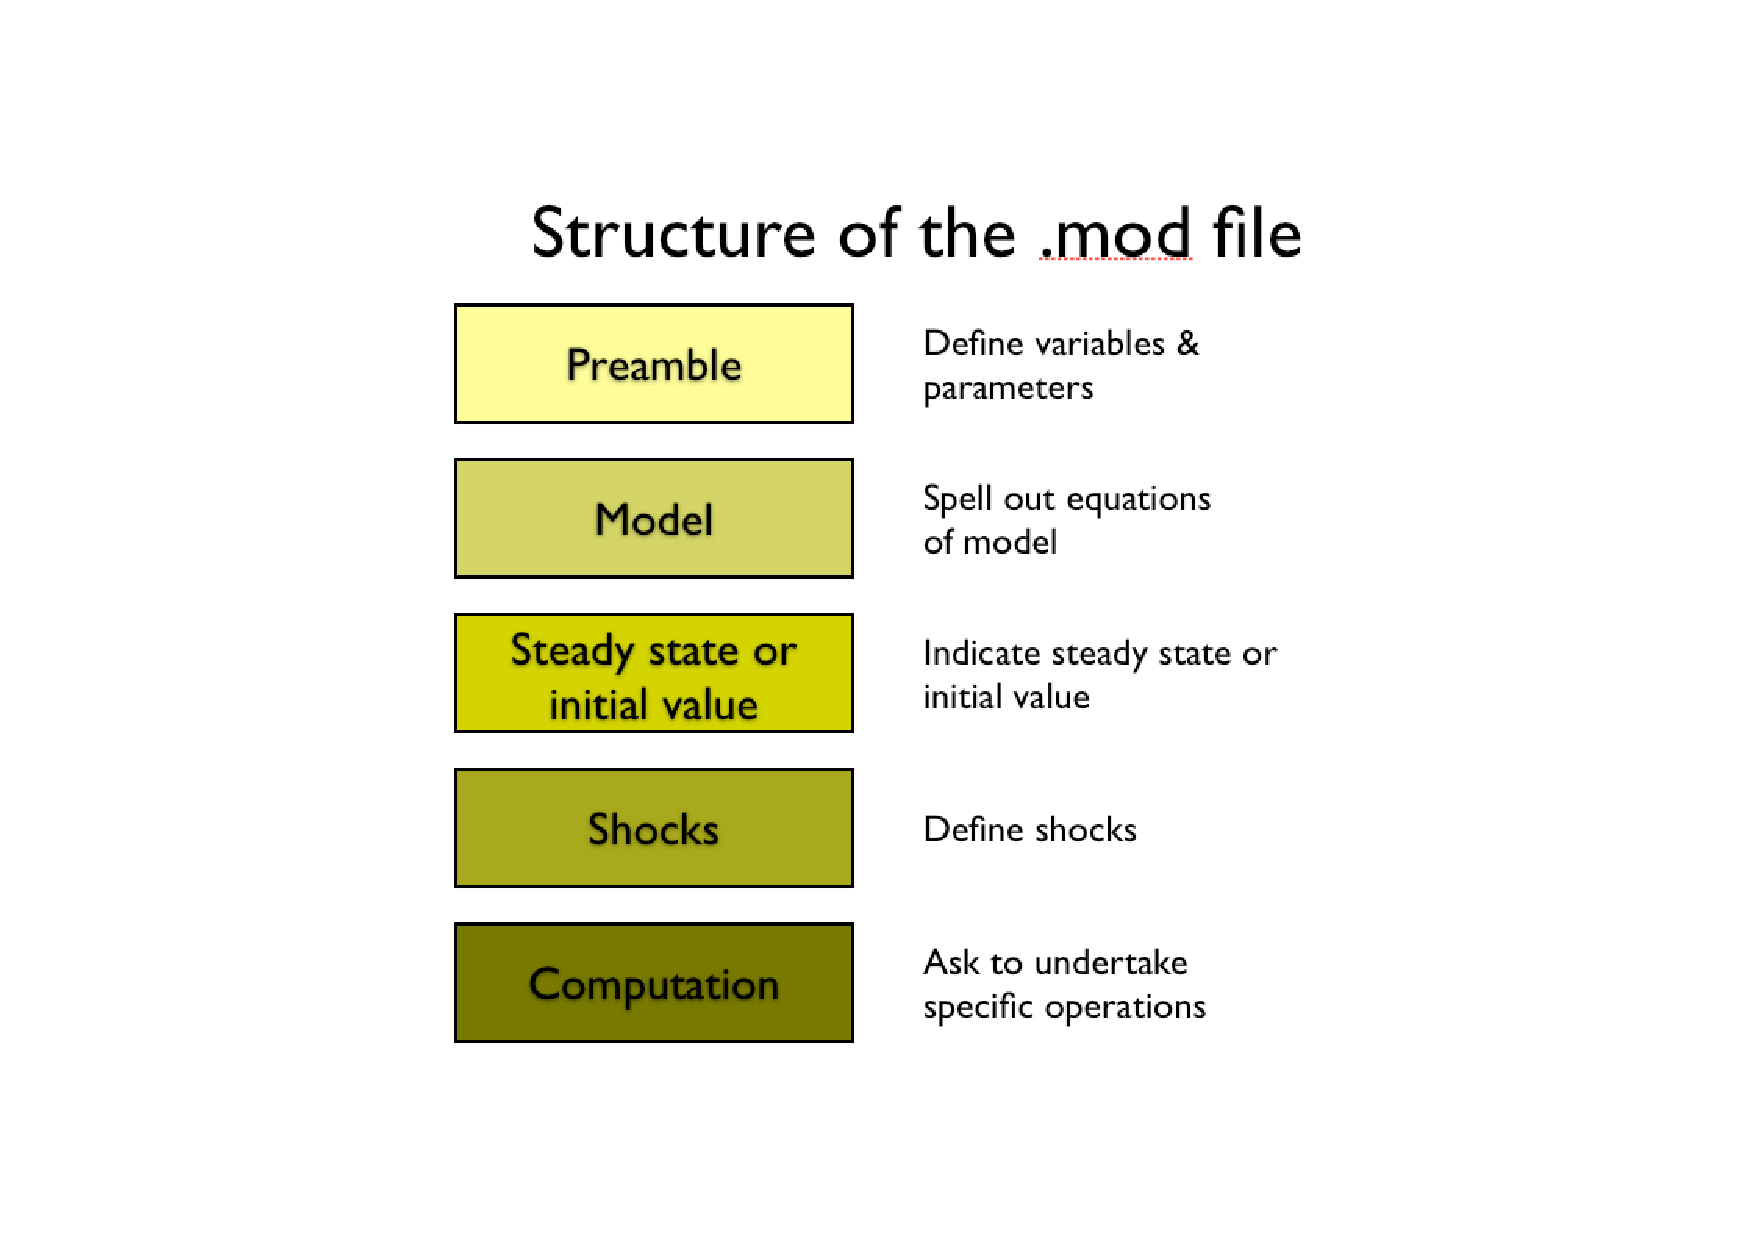
\includegraphics[width=1.0\textwidth]{P_ModStruct5} 
\end{center} 
\caption[Structure of the .mod file]{The .mod file contains five logically distinct parts.} 
\end{figure}

\section{Filling out the preamble} \label{sec:preamble}
The preamble generally involves three commands that tell Dynare what are the model's variables, which are endogenous and what are the parameters. The \textbf{commands} are:
\begin{itemize}
\item \texttt{var} starts the list of endogenous variables, to be separated by commas. 
\item \texttt{varexo} starts the list of exogenous variables that will be shocked.
\item \texttt{parameters} starts the list of parameters and assigns values to each.
\end{itemize}
In the case of our example, let's differentiate between the stochastic and deterministic cases. First, we lay these out, then we discuss them. 

\subsection{The deterministic case}
The model is inherited exactly as specified in the earlier description, except that we no longer need the $e_t$ variable, as we can make $z_t$ directly exogenous. Thus, the \textbf{preamble would look like}:\\
\\
\texttt{var y c k i l y\_l w r;\\
varexo z;\\
parameters beta psi delta alpha sigma epsilon;\\
alpha   = 0.33;\\
beta    = 0.99;\\
delta   = 0.023;\\
psi     = 1.75;\\
sigma   = (0.007/(1-alpha));\\
epsilon = 10;}\\

\subsection{The stochastic case}
In this case, we go back to considering the law of motion for technology, consisting of an exogenous shock, $e_t$. With respect to the above, we therefore adjust the list of endogenous and exogenous variables, and add the parameter $\rho$. Here's what the \textbf{preamble would look like}:\\ 
\\
\texttt{var y c k i l y\_l w r  z;\\
varexo e;\\
parameters beta psi delta alpha rho sigma epsilon;\\
alpha   = 0.33;\\
beta    = 0.99;\\
delta   = 0.023;\\
psi     = 1.75;\\
rho     = 0.95; \\ 
sigma   = (0.007/(1-alpha));\\
epsilon = 10;}\\

\subsection{Comments on your first lines of Dynare code}

As you can tell, writing a .mod file is really quite straightforward. Two quick comments:\\

\textsf{\textbf{NOTE!}} Remember that each instruction of the .mod file must be terminated by a semicolon (;), although a single instruction can span two lines if you need extra space (just don't put a semicolon at the end of the first line).\\

\textsf{\textbf{TIP!}} You can also comment out any line by starting the line with two forward slashes (//), or comment out an entire section by starting the section with /* and ending with */. For example:\\
\\
\texttt{var y c k i l y\_l w r  z;\\
varexo e;\\
parameters beta psi delta \\
alpha rho sigma epsilon;\\
// the above instruction reads over two lines\\
/*\\
the following section lists\\
several parameters which were\\
calibrated by my co-author. Ask\\
her all the difficult questions!\\
*/\\
alpha   = 0.33;\\
beta    = 0.99;\\
delta   = 0.023;\\
psi     = 1.75;\\
rho     = 0.95; \\ 
sigma   = (0.007/(1-alpha));\\
epsilon = 10;}\\  
\\

\section{Specifying the model} \label{sec:modspe}
\subsection{Model in Dynare notation}
One of the beauties of Dynare is that you can \textbf{input your model's equations naturally}, almost as if you were writing them in an academic paper. This greatly facilitates the sharing of your Dynare files, as your colleagues will be able to understand your code in no-time. There are just a few conventions to follow. Let's first have a look at our \textbf{model in Dynare notation}, and then go through the various Dynare input conventions. What you can already try to do is glance at the model block below and see if you can recognize the equations from the earlier example. See how easy it is to read Dynare code? \\
\\
\texttt{model;\\
  (1/c) = beta*(1/c(+1))*(1+r(+1)-delta);\\
  psi*c/(1-l) = w;\\
  c+i = y;\\
  y = (k(-1)$\hat{}$alpha)*(exp(z)*l)$\hat{}$(1-alpha);\\
  w = y*((epsilon-1)/epsilon)*(1-alpha)/l;\\
  r = y*((epsilon-1)/epsilon)*alpha/k(-1);\\
  i = k-(1-delta)*k(-1);\\
  y\_l = y/l;\\
  z = rho*z(-1)+e;\\
end;}\\

Just in case you need a hint or two to recognize these equations, here's a brief description: the first equation is the Euler equation in consumption. The second the labor supply function. The third the accounting identity. The fourth is the production function. The fifth and sixth are the marginal cost equal to markup equations. The seventh is the investment equality. The eighth an identity that may be useful and the last the equation of motion of technology.

\textsf{\textbf{NOTE!}} that the above model specification corresponds to the \textbf{stochastic case}; indeed, notice that the law of motion for technology is included, as per our discussion of the preamble. The corresponding model for the \textbf{deterministic casce} would simply loose the last equation. 

\subsection{General conventions}
The above example illustrates the use of a few important commands and conventions to translate a model into a Dynare-readable .mod file. 
\begin{itemize}
\item The first thing to notice, is that the model block of the .mod file begins with the command \texttt{model} and ends with the command \texttt{end}. 
\item Second, in between, there need to be as many equations as you declared endogenous variables (this is actually one of the first things that Dynare checks; it will immediately let you know if there are any problems). 
\item Third, as in the preamble and everywhere along the .mod file, each line of instruction ends with a semicolon (except when a line is too long and you want to break it across two lines. This is unlike Matlab where if you break a line you need to add \ldots). 
\item Fourth, equations are entered one after the other; no matrix representation is necessary. Note that variable and parameter names used in the model block must be the same as those declared in the preamble; \textsf{\textbf{TIP!}} remember that variable and parameter names are case sensitive. 
\end{itemize}

\subsection{Notational conventions}

\begin{itemize}
\item Variables entering the system with a time $t$ subscript are written plainly. For example, $x_t$ would be written $x$. 
\item Variables entering the system with a time $t-n$ subscript are written with $(-n)$ following them. For example, $x_{t-2}$ would be written $x(-2)$ (incidentally, this would count as two backward looking variables). 
\item In the same way, variables entering the system with a time $t+n$ subscript are written with $(+n)$ following them. For example, $x_{t+2}$ would be written $x(+2)$. Writing $x(2)$ is also allowed, but this notation makes it slightly harder to count by hand the number of forward looking variables (a useful measure to check); more on this below \ldots
\end{itemize}

\subsection{Timing conventions}
\begin{itemize}
\item In Dynare, the timing of each variable reflects when that variable is decided. For instance, our capital stock is not decided today, but yesterday (recall that it is a function of yesterday's investment and capital stock); it is what we call in the jargon a \textbf{predetermined} variable. Thus, eventhough in the example presented above we wrote $k_{t+1}=i_t + (1-\delta)k_t$, as in many papers, we would translate this equation into Dynare as \texttt{k=i+(1-delta)*k(-1)}.
\item As another example, consider that in some wage negociation models, wages used during a period are set the period before. Thus, in the equation for wages, you can write wage in period $t$ (when they are set), but in the labor demand equation, wages should appear with a one period lag.
\item A slightly more roundabout way to explain the same thing is that for stock variables, you must use a ``stock at the end of the period'' concept. It is investment during period $t$ that sets stock at the end of period $t$. Be careful, a lot of papers use the ``stock at the beginning of the period'' convention, as we did (on purpose to highlight this distinction!) in the setup of the example model above. 
\end{itemize}

\subsection{Conventions specifying non-predetermined variables}
\begin{itemize}
\item A (+1) next to a variable tells Dynare to count the occurrence of that variable as a jumper or forward-looking or non-predetermined variable. 
\item \textbf{Blanchard-Kahn} conditions are met only if the number of non-predetermined variables equals the number of eigenvalues greater than one. If this condition is not met, Dynare will put up a warning. 
\item Note that a variable may occur both as predetermined and non-predetermined. For instance, consumption could appear with a lead in the Euler equation, but also with a lag in a habit formation equation, if you had one. In this case, the second order difference equation would have two eigenvalues, one needing to be greater and the other smaller than one for stability. 
\end{itemize}

\subsection{Linear and log-linearized models}
There are two other variants of the system's equations which Dynare accommodates. First, the \textbf{linear model} and second, the \textbf{model in exp-logs}. In the first case, all that is necessary is to write the term \texttt{(linear)} next to the command \texttt{model}. Our example, with just the equation for $y_l$ for illustration, would look like:\\
\\
\texttt{model (linear);\\
yy\_l=yy - ll;\\
end;}\\
\\
where repeating a letter for a variable means difference from steady state.\\

Otherwise, you may be interested to have Dynare take Taylor series expansions in logs rather than in levels; this turns out to be a very useful option when estimating models with unit roots, as we will see in chapter \ref{ch:estbase}. If so, simply rewrite your equations by taking the exponential and logarithm of each variable. The Dynare input convention makes this very easy to do. Our example would need to be re-written as follows (just shown for the first two equations)\\
\\
\texttt{model;\\
  (1/exp(cc)) = beta*(1/exp(cc(+1)))*(1+exp(rr(+1))-delta);\\
  psi*exp(cc)/(1-exp(ll)) = exp(ww);\\
  end;}\\
  \\
  where, this time, repeating a letter for a variable means log of that variable, so that the level of a variable is given by $exp(repeated variable)$.

\section{Specifying steady states and/or initial values} \label{sec:ssshock}
Material in this section has created much confusion in the past. But with some attention to the explanations below, you should get through unscathed. Let's start by emphasizing the uses of this section of the .mod file. First, recall that stochastic models need to be linearized. Thus, they need to have a steady state. One of the functions of this section is indeed to provide these steady state values, or approximations of values. Second, irrespective of whether you're working with a stochastic or deterministic model, you may be interested to start your simulations or impulse response functions from either a steady state, or another given point. This section is also useful to specify this starting value. Let's see in more details how all this works.\\

In passing, though, note that the relevant commands in this section are \texttt{initval}, \texttt{endval} or, more rarely, \texttt{histval} which is covered only in the \href{http://www.dynare.org/documentation-and-support/manual}{Reference Manual}. The first two are instead covered in what follows. \\

\subsection{Stochastic models and steady states}
In a stochastic setting, your model will need to be linearized before it is solved. To do so, Dynare needs to know your model's steady state (more details on finding a steady state, as well as tips to do so more efficiently, are provided in section \ref{sec:findsteady} below). You can either enter exact steady state values into your .mod file, or just approximations and let Dynare find the exact steady state (which it will do using numerical methods based on your approximations). In either case, these values are entered in the \texttt{initval} block, as in the following fashion: \\
\\
\texttt{initval;\\
  k = 9;\\
  c = 0.7;\\
  l = 0.3;\\
  w = 2.0;\\
  r = 0;\\
  z = 0; \\
  e = 0;\\
end;}
\\

Then, by using the command \texttt{steady}, you can control whether you want to start your simulations or impulse response functions from the steady state, or from the exact values you specified in the \texttt{initval} block. Adding \texttt{steady} just after your \texttt{initval} block will instruct Dynare to consider your initial values as mere approximations and start simulations or impulse response functions from the exact steady state. On the contrary, if you don't add the command \texttt{steady}, your simulations or impulse response functions will start from your initial values, even if Dynare will have calculated your model's exact steady state for the purpose of linearization. \\

For the case in which you would like simulations and impulse response functions to begin at the steady state, the above block would be expanded to yield:\\
\\
\texttt{initval;\\
  k = 9;\\
  c = 0.7;\\
  l = 0.3;\\
  w = 2.0;\\
  r = 0;\\
  z = 0; \\
  e = 0;\\
end;\\
\\
steady;}
\\

\textsf{\textbf{TIP!}} If you're dealing with a stochastic model, remember that its linear approximation is good only in the vicinity of the steady state, thus it is strongly recommended that you start your simulations from a steady state; this means either using the command \texttt{steady} or entering exact steady state values. \\


\subsection{Deterministic models and initial values}
Deterministic models do not need to be linearized in order to be solved. Thus, technically, you do not need to provide a steady state for these model. But practically, most researchers are still interested to see how a model reacts to shocks when originally in steady state. In the deterministic case, the \texttt{initval} block serves very similar functions as described above. If you wanted to shock your model starting from a steady state value, you would enter approximate (or exact) steady state values in the \texttt{initval} block, followed by the command \texttt{steady}. Otherwise, if you wanted to begin your solution path from an arbitrary point, you would enter those values in your \texttt{initval} block and not use the \texttt{steady} command. An illustration of the \texttt{initval} block in the deterministic case appears further below. \\

\subsection{Finding a steady state} \label{sec:findsteady}

The difficulty in the above, of course, is calculating actual steady state values. Doing so borders on a form of art, and luck is unfortunately part of the equation. Yet, the following \textsf{\textbf{TIPS!}} may help.\\

As mentioned above, Dynare can help in finding your model's steady state by calling the appropriate Matlab functions. But it is usually only successful if the initial values you entered are close to the true steady state. If you have trouble finding the steady state of your model, you can begin by playing with the \textbf{options following the \texttt{steady} command}. These are:
\begin{itemize}
\item \texttt{solve\_algo = 0}: uses Matlab Optimization Toolbox FSOLVE
\item \texttt{solve\_algo = 1}: uses Dynare�s own nonlinear equation solver
\item \texttt{solve\_algo = 2}: splits the model into recursive blocks and solves each block in turn. 
\item \texttt{solve\_algo = 3}: uses the Sims solver. This is the default option if none are specified.
\end{itemize}

For complicated models, finding suitable initial values for the endogenous variables is the trickiest part of finding the equilibrium of that model. Often, it is better to start with a smaller model and add new variables one by one.\\

But even for simpler models, you may still run into difficulties in finding your steady state. If so, another option is to \textbf{enter your model in linear terms}. In this case, variables would be expressed in percent deviations from steady state. Thus, their initial values would all be zero. Unfortunately, if any of your original (non-linear) equations involve sums (a likely fact), your linearized equations will include ratios of steady state values, which you would still need to calculate. Yet, you may be left needing to calculate fewer steady state values than in the original, non-linear, model. \\

Alternatively, you could also use an \textbf{external program to calculate exact steady state values}. For instance, you could write an external \textbf{Maple} file and then enter the steady state solution by hand in Dynare. But of course, this procedure could be time consuming and bothersome, especially if you want to alter parameter values (and thus steady states) to undertake robustness checks. \\

The alternative is to write a \textbf{Matlab} program to find your model's steady state. Doing so has the clear advantages of being able to incorporate your Matlab program directly into your .mod file so that running loops with different parameter values, for instance, becomes seamless. \textsf{\textbf{NOTE!}} When doing so, your matlab (.m) file should have the same name as your .mod file, followed by \texttt{\_steadystate} For instance, if your .mod file is called \texttt{example.mod}, your Matlab file should be called \texttt{example\_steadystate.m} and should be saved in the same directory as your .mod file. Dynare will automatically check the directory where you've saved your .mod file to see if such a Matlab file exists. If so, it will use that file to find steady state values regardless of whether you've provided initial values in your .mod file. \\

Because Matlab does not work with analytical expressions, though (unless you're working with a particular toolbox), you need to do a little work to write your steady state program. It is not enough to simply input the equations as you've written them in your .mod file and ask Matlab to solve the system. You will instead need to write your steady state program as if you were solving for the steady state by hand. That is, you need to input your expressions sequentially, whereby each left-hand side variable is written in terms of known parameters or variables already solved in the lines above. For example, the steady state file corresponding to the above example, in the stochastic case, would be: (** example file to be added shortly) \\

\subsection{Checking system stability}
\textsf{\textbf{TIP!}} A handy command that you can add after the \texttt{initval} or \texttt{endval} block (following the \texttt{steady} command if you decide to add one) is the \texttt{check} command. This \textbf{computes and displays the eigenvalues of your system} which are used in the solution method. As mentioned earlier, a necessary condition for the uniqueness of a stable equilibrium in the neighborhood of the steady state is that there are 
as many eigenvalues larger than one in modulus as there are forward looking variables in the system. If this condition is not met, Dynare will tell you that the Blanchard-Kahn conditions are not satisfied (whether or not you insert the \texttt{check} command). \\


\section{Adding shocks}

\begin{comment}
\begin{figure} \label{fig:shockmodel}
\begin{center} 
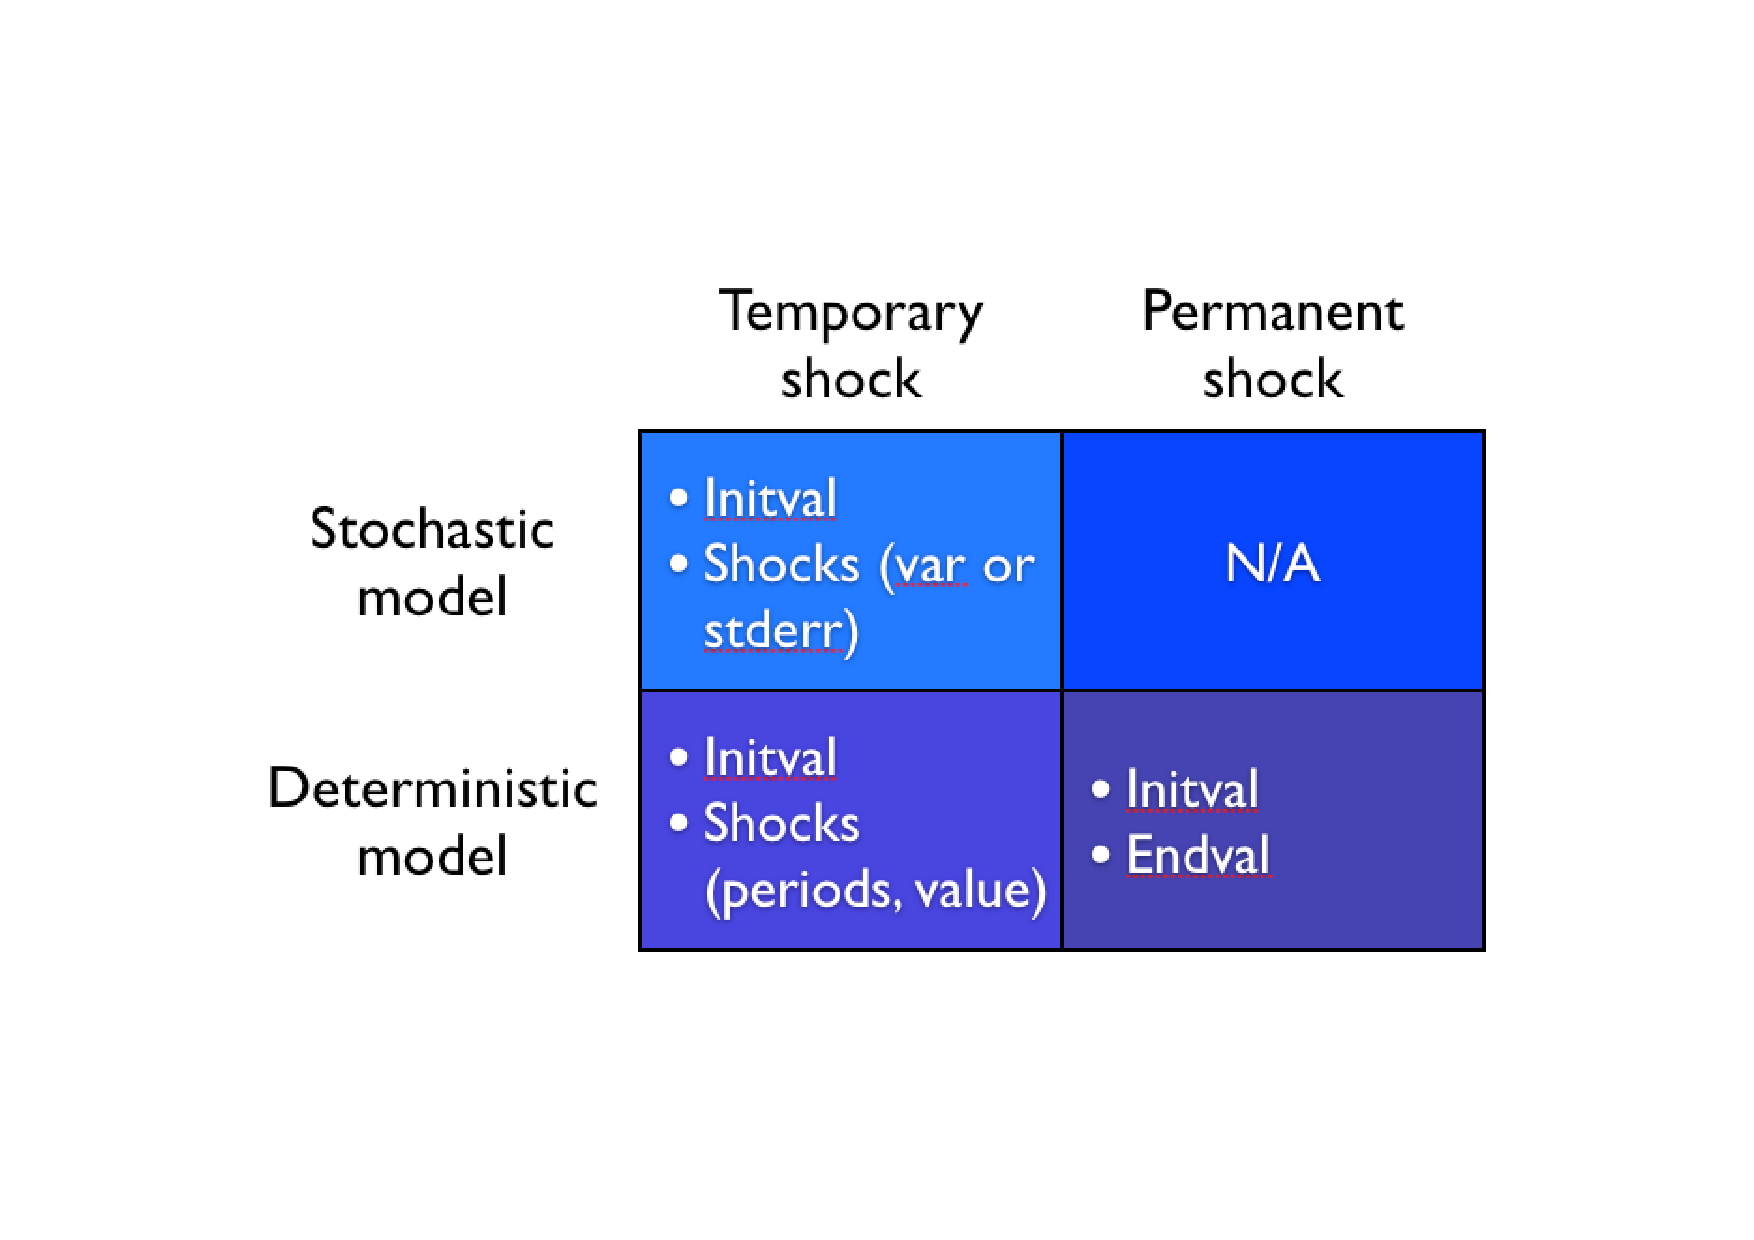
\includegraphics[width=1.0\textwidth]{P_ShockModel2} 
\end{center} 
\caption[Shock and model-type matrix]{Depending on the model type you're working with and the desired shocks, you will need to mix and match the various steady state and shock commands.} 
\end{figure}
\end{comment}

\subsection{Deterministic models - temporary shocks}
When working with a deterministic model, you have the choice of introducing both temporary and permanent shocks. The distinction is that under a temporary shock, the model eventually comes back to steady state, while under a permanent shock, the model reaches a new steady state. In both cases, though, the shocks are entirely expected, as explained in our original discussion on stochastic and deterministic models. \\

To work with a \textbf{temporary shock}, you are free to set the duration and level of the shock. To specify a shock that lasts 9 periods on $z_t$, for instance, you would write:\\
\\
\texttt{shocks;\\
var z;\\
periods 1:9;\\
values 0.1;\\
end;}\\

Given the above instructions, Dynare would replace the value of $z_t$ specified in the \texttt{initval} block with the value of 0.1 entered above. If variables were in logs, this would have corresponded to a 10\% shock. Note that you can also use the \texttt{mshocks} command which multiplies the initial value of an exogenous variable by the \texttt{mshocks} value. Finally, note that we could have entered future periods in the shocks block, such as \texttt{periods 5:10}, in order to study the anticipatory behavior of agents in response to future shocks.\\

\subsection{Deterministic models - permanent shocks}
To study the effects of a \textbf{permanent shock} hitting the economy today, such as a structural change in your model, you would not specify actual ``shocks'', but would simply tell the system to which (steady state) values you would like it to move and let Dynare calculate the transition path. To do so, you would use the \texttt{endval} block following the usual \texttt{initval} block. For instance, you may specify all values to remain common between the two blocks, except for the value of technology which you may presume changes permanently. The corresponding instructions would be:\\
\\
\texttt{initval;\\
  k = 9;\\
  c = 0.7;\\
  l = 0.3;\\
  w = 2.0;\\
  r = 0;\\
  z = 0; \\
end;\\
steady;\\
\\
endval;\\
  k = 9;\\
  c = 0.7;\\
  l = 0.3;\\
  w = 2.0;\\
  r = 0;\\
  z = 0.1; \\
end;\\
steady;}\\
\\
where \texttt{steady} can also be added to the \texttt{endval} block, and serves the same functionality as described earlier (namely, of telling Dynare to start and/ or end at a steady state close to the values you entered. If you do not use \texttt{steady} after \texttt{endval}, and the latter does not list exact steady state values, you may impose on your system that it does not return to steady state. This is unusual. In this case, your problem would become a so-called two boundary problem, which, when solved, requires that the path of your endogenous variables pass through the steady state closest to your \texttt{endval} values). In our example, we make use of the second \texttt{steady} since the actual terminal steady state values are bound to be somewhat different from those entered above, which are nothing but the initial values for all variables except for technology.\\

In the above example, the value of technology would move to 0.1 in period 1 (tomorrow) and thereafter. But of course, the other variables - the endogenous variables - will take longer to reach their new steady state values. \textsf{\textbf{TIP!}} If you instead wanted to study the effects of a permanent but future shock (anticipated as usual), you would have to add a \texttt{shocks} block after the \texttt{endval} block to ``undo'' the first several periods of the permanent shock. For instance, suppose you wanted the value of technology to move to 0.1, but only in period 10. Then you would follow the above \texttt{endval} block with:\\
\\
\texttt{shocks;\\
var z;\\
periods 1:9;\\
values 0;\\
end;}\\

\subsection{Stochastic models}

Recall from our earlier description of stochastic models that shocks are only allowed to be temporary. A permanent shock cannot be accommodated due to the need to stationarize the model around a steady state. Furthermore, shocks can only hit the system today, as the expectation of future shocks must be zero. With that in mind, we can however make the effect of the shock propagate slowly throughout the economy by introducing a ``latent shock variable'' such as $e_t$ in our example, that affects the model's true exogenous variable, $z_t$ in our example, which is itself an $AR(1)$, exactly as in the model we introduced from the outset. In that case, though, we would declare $z_t$ as an endogenous variable and $e_t$ as an exogenous variable, as we did in the preamble of the .mod file in section \ref{sec:preamble}. Supposing we wanted to add a shock with variance $\sigma^2$, where $\sigma$ is determined in the preamble block, we would write: \\
\\
\texttt{shocks;\\
var e = sigma $\widehat{}$ 2;\\
end;}\\
\\

\textsf{\textbf{TIP!}} You can actually \textbf{mix in deterministic shocks} in stochastic models by using the commands \texttt{varexo\_det} and listing some shocks as lasting more than one period in the \texttt{shocks} block. For information on how to do so, please see the \href{http://www.dynare.org/documentation-and-support/manual}{Reference Manual}. This can be particularly useful if you're studying the effects of anticipated shocks in a stochastic model. For instance, you may be interested in what happens to your monetary model if agents began expecting higher inflation, or a depreciation of your currency. \\

\section{Selecting a computation} \label{sec:compute}
So far, we have written an instructive .mod file, but what should Dynare do with it? What are we interested in? In most cases, it will be impulse response functions (IRFs) due to the external shocks. Let's see which are the appropriate commands to give to Dynare. Again, we will distinguish between deterministic and stochastic models. \\

\subsection{For deterministic models}
In the deterministic case, all you need to do is add the command \texttt{simul} at the bottom of your .mod file. Note that the command takes the option \mbox{\texttt{[ (periods=INTEGER) ] }} The command \texttt{simul} triggers the computation a numerical simulation of the trajectory of the model's solution for the number of periods set in the option. To do so, it uses a Newton method to solve simultaneously all the equations for every period (see \citet{Juillard1996} for details). Note that unless you use the \texttt{endval} command, the algorithm makes the simplifying assumption that the system is back to equilibrium after the specified number of periods. Thus, you must specify a large enough number of periods such that increasing it further doesn't change the simulation for all practical purpose. In the case of a temporary shock, for instance, the trajectory will basicaly describe how the system gets back to equilibrium after being perturbed from the shocks you entered.\\

\subsection{For stochastic models}
In the more common case of stochastic models, the command \texttt{stoch\_simul} is appropriate. This command instructs Dynare to compute a Taylor approximation of the decision and transition functions for the model (the equations listing current values of the endogenous variables of the model as a function of the previous state of the model and current shocks), impulse response 
functions and various descriptive statistics (moments, variance decomposition, correlation and autocorrelation coefficients).\footnote{For correlated shocks, the variance decomposition is computed as in the VAR literature through a Cholesky 
decomposition of the covariance matrix of the exogenous variables. When the shocks are correlated, the variance 
decomposition depends upon the order of the variables in the varexo command.}\\

Impulse response functions are the expected future path of the endogenous variables conditional on a shock in period 1 of one standard deviation.\textsf{\textbf{TIP!}} If you linearize your model up to a first order, impulse response functions are simply the algebraic forward iteration of your model's policy or decision rule. If you instead linearize to a second order, impulse response functions will be the result of actual Monte Carlo simulations of future shocks. This is because in second order linear equations, you will have cross terms involving the shocks, so that the effects of the shocks depend on the state of the system when the shocks hit. Thus, it is impossible to get algebraic average values of all future shocks and their impact. The technique is instead to pull future shocks from their distribution and see how they impact your system, and repeat this procedure a multitude of times in order to draw out an average response. That said, note that future shocks will not have a significant impact on your results, since they get averaged between each Monte Carlo trial and in the limit should sum to zero, given their mean of zero. Note that in the case of a second order approximation, Dynare will return the actual sample moments from the simulations. For first order linearizations, Dynare will instead report theoretical moments. In both cases, the return to steady state is asymptotic, \textsf{\textbf{TIP!}} thus you should make sure to specify sufficient periods in your IRFs such that you actually see your graphs return to steady state. Details on implementing this appear below.\\

If you're interested to peer a little further into what exactly is going on behind the scenes of Dynare's computations, have a look at Chapter \ref{ch:solbeh}. Here instead, we focus on the application of the command and reproduce below the most common options that can be added to \texttt{stoch\_simul}. For a complete list of options, please see the \href{http://www.dynare.org/documentation-and-support/manual}{Reference Manual}. \\

\textbf{Options following the \texttt{stoch\_simul} command:}
\begin{itemize}
\item ar = INTEGER: Order of autocorrelation coefficients to compute and to print (default = 5).
\item dr\_algo = 0 or 1: specifies the algorithm used for computing the quadratic approximation of the decision rules: $0$ uses a pure perturbation approach as in \citet{SchmittGrohe2004} (default) and 1 moves the point around which the Taylor expansion is computed toward the means of the distribution as in \citet{CollardJuillard2001a}.
\item drop = INTEGER: number of points dropped at the beginning of simulation before computing the summary 
statistics (default = 100).
\item hp\_filter = INTEGER: uses HP filter with lambda = INTEGER before computing moments (default: no filter).
\item hp\_ngrid = INTEGER: number of points in the grid for the discreet Inverse Fast Fourier Transform used in the 
HP filter computation. It may be necessary to increase it for highly autocorrelated processes (default = 512).
\item irf = INTEGER: number of periods on which to compute the IRFs (default = 40). Setting IRF=0, suppresses the 
plotting of IRF�s.  
\item relative\_irf requests the computation of normalized IRFs in percentage of the standard error of each shock.
\item nocorr: doesn�t print the correlation matrix (printing is the default).
\item nofunctions: doesn�t print the coefficients of the approximated solution (printing is the default). 
\item nomoments: doesn�t print moments of the endogenous variables (printing them is the default).
\item noprint: cancel any printing; usefull for loops. 
\item order = 1 or 2 : order of Taylor approximation (default = 2), unless you're working with a linear model in which case the order is automatically set to 1.  
\item periods = INTEGER: specifies the number of periods to use in simulations (default = 0). \textsf{\textbf{TIP!}} A simulation is similar to running impulse response functions with a model linearized to the second order, in the way that both sample shocks from their distribution to see how the system reacts, but a simulation only repeats the process once, whereas impulse response functions run a multitude of Monte Carlo trials in order to get an average response of your system. 
\item qz\_criterium = INTEGER or DOUBLE: value used to split stable from unstable eigenvalues in reordering the 
Generalized Schur decomposition used for solving 1st order problems (default = 1.000001).
\item replic = INTEGER: number of simulated series used to compute the IRFs (default = 1 if order = 1, and 50 
otherwise).
\item simul\_seed = INTEGER or DOUBLE or (EXPRESSION): specifies a seed for the random number generator so as to obtain the 
same random sample at each run of the program. Otherwise a different sample is used for each run (default: seed 
not specified). If you linearized to a second order, Dynare will actually undertake Monte Carlo simulations to generate moments of your variables. Because of the simulation, results are bound to be slightly different each time you run your program, except if you fix the seed for the random number generator. \textsf{\textbf{TIP!}} If you do decide to fix the seed, you should at least try to run your program without using \texttt{simul\_seed}, just to check the robustness of your results.
\end{itemize}

Going back to our good old example, suppose we were interested in printing all the various measures of moments of our variables, want to see impulse response functions for all variables, are basically happy with all default options and want to carry out simulations over a good number of periods. We would then end our .mod file with the following command:\\
\\
\texttt{stoch\_simul(periods=2100);}\\

\section{The complete .mod file}
For completion's sake, and for the pleasure of seeing our work bear its fruits, here are the complete .mod files corresponding to our example for the deterministic and stochastic case. You can find the corresponding files in the \textsl{models} folder under \textsl{UserGuide} in your installation of Dynare. The files are called \texttt{RBC\_Monop\_JFV.mod} for stochastic models and \texttt{RBC\_Monop\_Det.mod} for deterministic models. 

\subsection{The stochastic model}

\texttt{var y c k i l y\_l w r  z;\\
varexo e;\\
parameters beta psi delta alpha rho sigma epsilon;\\
alpha   = 0.33;\\
beta    = 0.99;\\
delta   = 0.023;\\
psi     = 1.75;\\
rho     = 0.95; \\ 
sigma   = (0.007\/(1-alpha));\\
epsilon = 10;\\
\\
model;\\
  (1/c) = beta*(1/c(+1))*(1+r(+1)-delta);\\
  psi*c/(1-l) = w;\\
  c+i = y;\\
  y = (k(-1)$\hat{}$alpha)*(exp(z)*l)$\hat{}$(1-alpha);\\
  w = y*((epsilon-1)/epsilon)*(1-alpha)/l;\\
  r = y*((epsilon-1)/epsilon)*alpha/k(-1);\\
  i = k-(1-delta)*k(-1);\\
  y\_l = y/l;\\
  z = rho*z(-1)+e;\\
end;\\
\\
initval;\\
  k = 9;\\
  c = 0.7;\\
  l = 0.3;\\
  w = 2.0;\\
  r = 0;\\
  z = 0; \\
  e = 0;\\
end;\\
\\
steady;\\
\\
check;\\
\\
shocks;\\
var e = sigma $\widehat{}$ 2;\\
end;\\
\\
stoch\_simul(periods=2100);}\\

\subsection{The deterministic model (case of temporary shock)}

\texttt{var y c k i l y\_l w r ;\\
varexo z;\\
parameters beta psi delta alpha sigma epsilon;\\
alpha   = 0.33;\\
beta    = 0.99;\\
delta   = 0.023;\\
psi     = 1.75;\\
sigma   = (0.007\/(1-alpha));\\
epsilon = 10;\\
\\
model;\\
  (1/c) = beta*(1/c(+1))*(1+r(+1)-delta);\\
  psi*c/(1-l) = w;\\
  c+i = y;\\
  y = (k(-1)$\hat{}$alpha)*(exp(z)*l)$\hat{}$(1-alpha);\\
  w = y*((epsilon-1)/epsilon)*(1-alpha)/l;\\
  r = y*((epsilon-1)/epsilon)*alpha/k(-1);\\
  i = k-(1-delta)*k(-1);\\
  y\_l = y/l;\\
end;\\
\\
initval;\\
  k = 9;\\
  c = 0.7;\\
  l = 0.3;\\
  w = 2.0;\\
  r = 0;\\
  z = 0; \\
end;\\
\\
steady;\\
\\
check;\\
\\
shocks;\\
var z;
periods 1:9;\\
values 0.1;\\
end;\\
\\
simul(periods=2100);}\\

\section{File execution and results}
To see this all come to life, let's run our .mod file, which is conveniently installed by default in the Dynare ``examples'' directory (the .mod file corresponding to the stochastic model is called RBC\_Monop\_JFV.mod and that corresponding to the deterministic model is called RBC\_Monop\_Det.mod). (** note, this may not be the case when testing the beta version of Matlab version 4) \\

\textbf{To run a .mod file}, navigate within Matlab to the directory where the example .mod files are stored. You can do this by clicking in the ``current directory'' window of Matlab, or typing the path directly in the top white field of Matlab. Once there, all you need to do is place your cursor in the Matlab command window and type, for instance, \texttt{dynare ExSolStoch;} to execute your .mod file. \\

Running these .mod files should take at most 30 seconds. As a result, you should get two forms of output - tabular in the Matlab command window and graphical in one or more pop-up windows. Let's review these results.\\

\subsection{Results - stochastic models}
\textbf{The tabular results} can be summarized as follows:
\begin{enumerate}
\item \textbf{Model summary:} a count of the various variable types in your model (endogenous, jumpers, etc...).
\item \textbf{Eigenvalues} should be displayed, and you should see a confirmation of the Blanchard-Kahn conditions if you used the command \texttt{check} in your .mod file. 
\item \textbf{Matrix of covariance of exogenous shocks:} this should square with the values of the shock variances and co-variances you provided in the .mod file.
\item \textbf{Policy and transition functions:} Solving the rational exectation model, $\mathbb{E}_t[f(y_{t+1},y_t,y_{t-1},u_t)]=0$ , means finding an unkown function, $y_t = g(y_{t-1},u_t)$  that could be plugged into the original model and satisfy the implied restrictions (the first order conditions). A first order approximation of this function can be written as $y_t = \bar{y} + g_y \hat{y}_{t-1} + g_u u_t$, with $\hat{y}_t = y_t-\bar{y}$ and $\bar{y}$ being the steadystate value of $y$, and where $g_x$ is the partial derivative of the $g$ function with respect to variable $x$. In other words, the function $g$ is a time recursive (approximated) representation of the model that can generate timeseries that will approximatively satisfy the rational expectation hypothesis contained in the original model. In Dynare, the table ``Policy and Transition function'' contains the elements of $g_y$ and $g_u$. Details on the policy and transition function can be found in Chapter \ref{ch:estadv}.
\item \textbf{Moments of simulated variables:} up to the fourth moments.
\item \textbf{Correlation of simulated variables:} these are the contemporaneous correlations, presented in a table.
\item \textbf{Autocorrelation of simulated variables:} up to the fifth lag, as specified in the options of \texttt{stoch\_simul}. 
\end{enumerate}

\textbf{The graphical results}, instead, show the actual impulse response functions for each of the endogenous variables, given that they actually moved. These can be especially useful in visualizing the shape of the transition functions and the extent to which each variable is affected. \textsf{\textbf{TIP!}} If some variables do not return to their steady state, either check that you have included enough periods in your simulations, or make sure that your model is stationary, i.e. that your steady state actually exists and is stable. If not, you should detrend your variables and rewrite your model in terms of those variables. 

\subsection{Results - deterministic models}
Automatically displayed results are much more scarce in the case of deterministic models. If you entered \texttt{steady}, you will get a list of your steady state results. If you entered \texttt{check}, eigenvalues will also be displayed and you should receive a statement that the rank condition has been satisfied, if all goes well! Finally, you will see some intermediate output: the errors at each iteration of the Newton solver used to estimate the solution to your model. \textsf{\textbf{TIP!}} You should see these errors decrease upon each iteration; if not, your model will probably not converge. If so, you may want to try to increase the periods for the transition to the new steady state (the number of simulations periods). But more often, it may be a good idea to revise your equations. Of course, although Dynare does not display a rich set of statistics and graphs corresponding to the simulated output, it does not mean that you cannot create these by hand from Matlab. To do so, you should start by looking at section \ref{sec:FindOut} of chapter \ref{ch:soladv} on finding, saving and viewing your output. 











